
\newpage
\section*{The Coq library}

\ocwsection \label{library}
This chapter describes the \Coq\ library, which is made of two parts:
\begin{itemize}
  \item a general mechanism to keep a trace of all operations and of
    the state of the system, with backtrack capabilities;
  \item a global environment for the CCI, with functions to export and 
    import compiled modules.
\end{itemize}
The modules of the library are organized as follows.

\bigskip
\begin{center}\epsfig{file=library.dep.ps}\end{center}
